\documentclass{beamer}
\usepackage[utf8]{inputenc}
\usepackage[T1]{fontenc}
\usepackage{import}

\usetheme{default}
\usecolortheme{seahorse}
\usefonttheme{serif}

\input{../preamble}

\title{PHGN 200 --- Electromagnetism and Optics}
\subtitle{Block III: Magnetics}

\author{}
\date{Block III Review Slides}

\begin{document}

\frame{\titlepage}

\begin{frame}{A Quick Introduction}

\begin{center}
    We learned in Block I that \emph{stationary charges} produce \emph{electric fields}.
\end{center}

\vfill

\begin{center}
    Then in Block II we learned that \emph{current} is nothing more than \emph{moving charges}.
\end{center}

\vfill

\begin{center}
    So what kind of fields do \emph{moving charges} produce? Magnetic fields!
\end{center}

\end{frame}

\begin{frame}{Biot-Savart Law}

The Biot-Savart Law reads

\begin{equation*}
    d\vec{B} = \frac{\mu_o I\ d\vec{\ell} \times \vec{r}}{4\pi\ r^3}
\end{equation*}

\vfill

\begin{center}
This gives us a recipe for finding magnetic fields from current-carrying wires.
\end{center}

\end{frame}

\begin{frame}{Worked Example --- A Current-Carrying Loop}

$\blacktriangleright$ Consider a loop of radius $R$ that carries a current $I$. What is the magnetic field at some point $P$ on the axis of the loop?

\begin{figure}[H]
\centering
\includegraphics[height=0.46\textheight]{figures/current_carrying_loop.png}
\end{figure}

\textit{Solution.} Let's start by building up all the pieces of the Biot-Savart law.

\begin{equation*}
    d\vec{B} = \frac{\mu_o I\ d\vec{\ell} \times \vec{r}}{4\pi\ r^3}
\end{equation*}

\end{frame}

\begin{frame}{Worked Example --- A Current-Carrying Loop}

Let's start with with $\vec{r}$-vector. As always, the $\vec{r}$-vector points from the source (the current-carrying loop) to the observation point.

\vfill

The observation point $P$ is situated on the $z$-axis. So its coordinates are $(0,0,z)$.

\end{frame}

\begin{frame}{Worked Example --- A Current-Carrying Loop}

\begin{figure}[H]
\centering
\includegraphics[height=0.8\textheight]{figures/loopy_bfield.png}
\end{figure}

\end{frame}

\begin{frame}{Worked Example --- A Current-Carrying Loop}

So the $\vec{r}$-vector is
\begin{gather*}
    \vec{r} = \left( 0 - R\cos{\theta} \right) \ihat + \left( 0 - R\sin{\theta} \right) \jhat + \left( z - 0 \right) \khat \\
    \boxed{\vec{r} = -R\cos{\theta}\ \ihat - R\sin{\theta}\ \jhat + z\ \khat}
\end{gather*}

and its magnitude is
\begin{align*}
    r &= \sqrt{\left( -R\cos{\theta} \right)^2 + \left( -R\sin{\theta} \right)^2 + \left( z \right)^2} \\
      &= \sqrt{R^2 \cos^2{\theta} + R^2 \sin^2{\theta} + z^2} \\
      &= \sqrt{R^2 \cancel{\left( \cos^2{\theta} + \sin^2{\theta} \right)} + z^2} \\
      &= \sqrt{R^2 + z^2}.
\end{align*}

\end{frame}

\begin{frame}{Worked Example --- A Current-Carrying Loop}

Now we need \textcolor{RED}{$d\vec{\ell}$}. This is the infinitesimal segment of the current-carrying wire.

\begin{figure}
\centering
\begin{tikzpicture}[scale=0.4]
    \draw[black, ->] (-6,0) -- (6,0) node[black, anchor=south west] {$x$};
    \draw[black, ->] (0,-6) -- (0,6) node[black, anchor=south west] {$y$};
    \draw[black, thick] (0,0) circle (4);
    %
    \draw[red, thick, ->] (4,0) -- (4,1);
    \draw[red, thick, ->] (2.828,2.828) -- (2.121,3.536);
    \draw[red, thick, ->] (0,4) -- (-1,4);
    \draw[red, thick, ->] (-2.828,2.828) -- (-3.536,2.121);
    \draw[red, thick, ->] (-4,0) -- (-4,-1);
    \draw[red, thick, ->] (-2.828,-2.828) -- (-2.121,-3.536);
    \draw[red, thick, ->] (0,-4) -- (1,-4);
    \draw[red, thick, ->] (2.828,-2.828) -- (3.536,-2.121);
\end{tikzpicture}
\end{figure}

\end{frame}

\begin{frame}{Worked Example --- A Current-Carrying Loop}

 We know that infinitesimal arc length is

\begin{equation*}
    \left| d\vec{\ell} \right| = d\ell = R\ d\theta
\end{equation*}

This holds for any circular path. However, if we want to get the components of the $d\vec{\ell}$ vector, we need to attenuate each term by the appropriate trig factor:

\begin{equation*}
    d\vec{\ell} = \left( \underbrace{\hspace{4em}}_{\parbox[c]{4em}{\centering \text{\tiny trig factor}}} R\ d\theta \right) \ihat + \left( \underbrace{\hspace{4em}}_{\parbox[c]{4em}{\centering \text{\tiny trig factor}}} R\ d\theta \right) \jhat
\end{equation*}

Finding which term goes like $\sin{\theta}$ and which goes like $\cos{\theta}$ is by far easiest to do with limiting values.

\end{frame}

\begin{frame}{Worked Example --- A Current-Carrying Loop}

\begin{equation*}
    d\vec{\ell} = \overbrace{\left( \underbrace{\hspace{4em}}_{\parbox[c]{4em}{\centering \text{\tiny trig factor}}} R\ d\theta \right)}^{dx} \ihat + \overbrace{\left( \underbrace{\hspace{4em}}_{\parbox[c]{4em}{\centering \text{\tiny trig factor}}} R\ d\theta \right)}^{dy} \jhat
\end{equation*}

At $\theta = \frac{\pi}{2}$, the $d\vec{\ell}$ vector points straight to the left. So we want a trig factor that respects $dy = 0$ when $\theta = \frac{\pi}{2}$. Immediately, this tells us that $dy = R\cos{\theta}\ d\theta$, since $\cos{\left(\frac{\pi}{2}\right)} = 0$. Conversely, we find that $dx = -R\sin{\theta}\ d\theta$, since the $d\vec{\ell}$ vector points to the left. So we have

\begin{equation*}
    \boxed{d\vec{\ell} = -R\sin{\theta}\ d\theta\ \ihat + R\cos{\theta}\ d\theta\ \jhat + 0\ \khat}
\end{equation*}

We can check this against the other limiting value, $\theta \to 0$. Indeed, we get
\begin{equation*}
    d\vec{\ell} \big|_{\theta = 0} = \cancelto{0}{-R\sin{(0)}\ d\theta\ \ihat} + {R\cos{(0)}\ d\theta\ \jhat} = R\ d\theta\ \jhat
\end{equation*}

\end{frame}

\begin{frame}{Worked Example --- A Current-Carrying Loop}

We can also start from first principles. We know, that $d\vec{\ell}$, in its most general form, is $d\vec{\ell} = dx\ \ihat + dy\ \jhat$. By convention, the positive $d\vec{\ell}$ vector points such that a counter-clockwise path is traced out along a circle. Moreover, we know that along a circle (with $\theta$ taken from the positive $x$-axis),
\begin{equation*}
    x = R\cos{\theta} \qquad \text{and} \qquad y = R\sin{\theta}.
\end{equation*}

Taking a derivative to get $dx$ and $dy$, we have
\begin{equation*}
    dx = -R\sin{\theta}\ d\theta \qquad \text{and} \qquad dy = R\cos{\theta}\ d\theta.
\end{equation*}

Putting everything together,
\begin{equation*}
    d\vec{\ell} = dx\ \ihat + dy\ \jhat = \boxed{-R\sin{\theta}\ d\theta\ \ihat + R\cos{\theta}\ d\theta\ \jhat}
\end{equation*}

\end{frame}

\begin{frame}{Worked Example --- A Current-Carrying Loop}

Now we need the cross-product $d\vec{\ell} \times \vec{r}$.

\begin{align*}
    d\vec{\ell} \times \vec{r} &= \begin{vmatrix} \ihat & \jhat & \khat \\ -R\sin{\theta}\ d\theta & R\cos{\theta}\ d\theta & 0 \\ -R\cos{\theta} & -R\sin{\theta} & z \end{vmatrix} \\
                               &= Rz\cos{\theta}\ d\theta\ \ihat + Rz\sin{\theta}\ d\theta\ \jhat\ + \\
                               &\textcolor{white}{white}\qquad\qquad\quad + \underbrace{\left( R^2 \sin^2{\theta}\ d\theta + R^2\cos^2{\theta}\ d\theta \right)}_{=\ R^2\ d\theta}\ \khat
\end{align*}

So we have
\begin{equation*}
    d\vec{\ell} \times \vec{r} = Rz\cos{\theta}\ d\theta\ \ihat + Rz\sin{\theta}\ d\theta\ \jhat + R^2\ d\theta\ \khat
\end{equation*}

\end{frame}

\begin{frame}{Worked Example --- A Current-Carrying Loop}

We don't care about the $\ihat$ or $\jhat$ components. Why?

\begin{equation*}
    d\vec{\ell} \times \vec{r} = \underbrace{Rz\cos{\theta}\ d\theta}_{\left( d\vec{\ell} \times \vec{r} \right)_x}\ \ihat + Rz\sin{\theta}\ d\theta\ \jhat + R^2\ d\theta\ \khat
\end{equation*}

\vfill

Say we want to determine the $\ihat$-component of the magnetic field. We would assemble the Biot-Savart law as usual:

\begin{equation*}
    B_x = \int dB_x = \bigintsss_{0}^{2\pi} \frac{\mu_o I\ \left( Rz\cos{\theta}\ d\theta \right)}{4\pi {\left( \sqrt{R^2 + z^2} \right)^3}}\ \ihat
\end{equation*}

We're integrating with respect to $\theta$. And everything in that integral barring $\cos{\theta}$ can be pulled out of the integral. But we know that $\displaystyle \int_{0}^{2\pi} \cos{\theta}\ d\theta = 0$.

\end{frame}

\begin{frame}{Worked Example --- A Current-Carrying Loop}

\begin{figure}[H]
\centering
\includegraphics[height=0.6\textheight]{figures/copper_loop.jpeg}
\end{figure}

\end{frame}

\begin{frame}{Worked Example --- A Current-Carrying Loop}

So now we know the magnetic field, on the axis of the loop, is strictly in the $\khat$ direction. Let's finish up by assembling the pieces of the Biot Savart law and integrating:

\begin{align*}
    \vec{B} = \int d\vec{B} &= \bigintss_{0}^{2\pi} \frac{\mu_o\ I\ \left( R^2\ d\theta \right)}{4\pi\ \left(R^2 + z^2\right)^{3/2}}\ \khat \\
                            &= \frac{\mu_o\ I\ R^2}{4\pi\ \left(R^2 + z^2 \right)^{3/2}} \cancelto{2\pi}{\int_{0}^{2\pi} d\theta}\ \khat
\end{align*}

And we end up with a familiar expression:
\begin{equation*}
    \boxed{\vec{B} = \frac{\mu_o I R^2}{2\left( R^2 + z^2 \right)^{3/2}}\ \khat} \blacktriangleleft
\end{equation*}

\end{frame}

\begin{frame}{Amp{\'e}re's Law}

Amp{\'e}re's law reads

\begin{equation*}
    \oint \vec{B} \cdot d\vec{\ell} = \mu_o I_{\text{thru}} + \underbrace{\cancel{\mu_o \epsilon_o \frac{d \Phi_E}{dt}}}_{\parbox[b]{5em}{\vspace{-0.5em} \begin{center} \tiny don't worry about displacement current \end{center}}}
\end{equation*}

\vfill

The left-hand side of Amp{\'e}re's law is a \emph{closed} line integral. Term of art: we integrate the magnetic field over an \emph{Amp{\'e}rian loop}.

\vfill

The right-hand side of Amp{\'e}re's law is the current enclosed by that Amp{\'e}rian loop. The most general method to determine enclosed current is to integrate the current density:
\begin{equation*}
    I_{\text{thru}} = \int \vec{J} \cdot d\vec{A} = \int J\ dA
\end{equation*}

\end{frame}

\begin{frame}{Remarks on Amp{\'e}re's Law}

Amp{\'e}re's law is a \emph{law of nature}. That is, it holds for \emph{any} closed loop. Consider, for instance, the current-carrying wire below.

\begin{figure}[H]
\centering
\includegraphics[height=0.6\textheight]{figures/infwire.png}
\end{figure}

\end{frame}

\begin{frame}{Remarks on Amp{\'e}re's Law}

The value of the integral $\displaystyle \oint \vec{B} \cdot d\vec{\ell}$ is the same whether the Amp{\'e}rian loop looks like this:

\begin{figure}[H]
\centering
\includegraphics[height=0.6\textheight]{figures/infwire_loop1.png}
\end{figure}

\end{frame}

\begin{frame}{Remarks on Amp{\'e}re's Law}

or like this:

\begin{figure}[H]
\centering
\includegraphics[height=0.6\textheight]{figures/infwire_loop2.png}
\end{figure}

Put another way, Amp{\'e}re's law --- the statement about the value of the integral $\displaystyle \oint \vec{B} \cdot d\vec{\ell}$ --- is true always, but is only useful sometimes.

\end{frame}

\begin{frame}{Using Amp{\'e}re's law to Solve for Magnetic Fields}

Under certain circumstances, the symmetry of a problem will enable us to solve for magnetic fields with Amp{\'e}re's law. If the magnetic field is always parallel to the $d\vec{\ell}$ vector of the Amp{\'e}rian loop, then
\begin{equation*}
    \oint \vec{B} \cdot d\vec{\ell} = \oint B\ d\ell,
\end{equation*}

since a dot product of parallel vectors is immaterial. Moreover, if the magnetic field is \emph{uniform} on the entirety of the loop then
\begin{equation*}
    \oint B\ d\ell = B \underbrace{\left( \oint d\ell \right)}_{\parbox[c]{3em}{\vspace{-0.5em}\begin{center} \tiny length of Amp{\'e}rian loop \end{center}}}
\end{equation*}

\end{frame}

\begin{frame}{Worked Example --- Using Amp{\'e}re's law to Solve for Magnetic Fields}

$\blacktriangleright$ A wire with radius $a$ carries a uniform current $I_o$. An annular cylinder with inner radius $b$ and outer radius $c$ is concentric with the inner wire, and carries a current such that its current density is given by $J_{\text{annular cylinder}} = \frac{1}{r^2}$ (assume the units on $J$ are \si{\ampere/\metre^2}). Find the magnitude of the magnetic field at a distance $r$ from the center axis, where

\begin{minipage}{0.4\textwidth}
\begin{flushleft}
\begin{figure}[H]
\centering
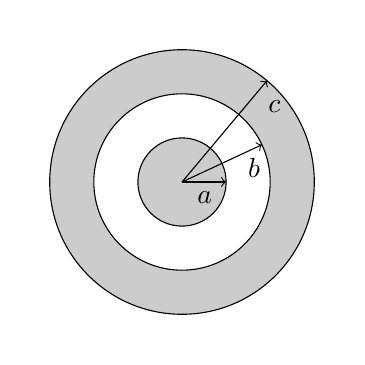
\begin{tikzpicture}[scale=0.28]
    % Draw annular cylinder
    \fill[white] (0,0) circle (7);
    \filldraw[color=black, fill=black!20] (0,0) circle (6);
    \filldraw[color=black, fill=black!0] (0,0) circle (4);
    % Draw inner conductor
    \filldraw[color=black, fill=black!20] (0,0) circle (2);
    % Radii on annular cylinder
    \draw[black, ->] (0:0) -- (50:6) node[black, pos=0.9, anchor=north west] {$c$};
    \draw[black, ->] (0:0) -- (25:4) node[black, pos=0.9, anchor=north] {$b$};
    \draw[black, ->] (0:0) -- (0:2) node[black, pos=0.9, anchor=north east] {$a$};
\end{tikzpicture}
\end{figure}
\end{flushleft}
\end{minipage}
~
\begin{minipage}{0.4\textwidth}
\begin{flushright}
\begin{enumerate}
    \item[(a)] $r < a$,
    \item[(b)] $a \leqslant r \leqslant b$,
    \item[(c)] $b \leqslant r \leqslant c$, and
    \item[(d)] $r > c$.
\end{enumerate}
\end{flushright}
\end{minipage}
\end{frame}

\begin{frame}{Worked Example --- Using Amp{\'e}re's law to Solve for Magnetic Fields}

\textit{Solution.} Amp{\'e}re's law reads

\begin{equation*}
    \oint \vec{B} \cdot d\vec{\ell} = \mu_o I_{\text{thru}}
\end{equation*}

We need the magnitude of the magnetic field at a distance $r$ from the center axis, where (a) $r < a$, (b) $a \leqslant r \leqslant b$, (c) $b \leqslant r \leqslant c$, and (d) $r > c$. For each of these, we'll need to calculate the the current enclosed.

\end{frame}

\begin{frame}{Worked Example --- Using Amp{\'e}re's law to Solve for Magnetic Fields}

\textbf{Part (a)}. Here the current enclosed by the Amp{\'e}rian loop is confined to the inner conductor, where the current is uniformly distributed. Therefore, it follows that the current density is $J = \frac{\text{total current}}{\text{total cross-sectional area}} = \frac{I}{\pi a^2}$. So the enclosed current is
\vspace{-1em}
\begin{align*}
    I_{\text{thru}} = \int J\ dA &= \overbrace{\left( \frac{I_o}{\pi a^2} \right)}^{J} \int dA \\
                                 &= \frac{I_o}{\pi a^2} \int_{0}^{r} 2\pi r'\ dr' \\
                                 &= \frac{2\pi I_o}{\pi a^2} \left( \frac{r'^2}{2} \right) \bigg|_{0}^{r} \\
                                 &= \frac{I_o\ r^2}{a^2}
\end{align*}

(The cross sectional area is a circle. So $A = \pi r^2$. Taking a derivative gives $dA = 2\pi r\ dr$.)

\end{frame}

\begin{frame}{Worked Example --- Using Amp{\'e}re's law to Solve for Magnetic Fields}

\textbf{Part (b)}. Here the Amp{\'e}rian loop is nested between the inner conductor and the outer conductor. There's no current in the region $a \leqslant r \leqslant b$, so the enclosed current is
\begin{align*}
    I_{\text{thru}} = \int J\ dA &= \overbrace{\left( \frac{I_o}{\pi a^2} \right)}^{J} \int dA \\
                                 &= \frac{I_o}{\pi a^2} \int_{0}^{a} 2\pi r'\ dr' \\
                                 &= \frac{I_o\ \cancel{a^2}}{\cancel{a^2}}
\end{align*}

That's reassuring. It should indeed be the case that the current through the Amp{\'e}rian loop is just the current carried by the inner wire.

\end{frame}

\begin{frame}{Worked Example --- Using Amp{\'e}re's law to Solve for Magnetic Fields}

\textbf{Part (c)}. Here the Amp{\'e}rian loop is nested inside the annular cylinder (the outer conductor), such that $b \leqslant r \leqslant c$. We're still enclosing the current from the inner conductor, but now we also have some current from the outer conductor, whose current density is given by the function $J_{\text{ann cyl}} = \frac{1}{r^2}$. As such, the enclosed current is
\begin{align*}
    I_{\text{thru}} &= I_o + \int_{b}^{r} \overbrace{\left( \frac{1}{r'^2} \right)}^{J_{\text{ann cyl}}} \overbrace{\left( 2\pi r'\ dr' \right)}^{dA} \\
    &= I_o + 2\pi \int_{b}^{r} \frac{dr'}{r'} \\
    &= I_o + 2\pi \ln{\left( \frac{r}{b} \right)}
\end{align*}

\end{frame}

\begin{frame}{Worked Example --- Using Amp{\'e}re's law to Solve for Magnetic Fields}

\textbf{Part (d)}. Here the Amp{\'e}rian loop is outside the annular cylinder, such that $r > c$. We're still enclosing the current from the inner conductor, but now we also have all of the  current from the outer conductor, whose current density is given by the function $J_{\text{ann cyl}} = \frac{1}{r^2}$. As such, the enclosed current is
\begin{align*}
    I_{\text{thru}} &= I_o + \int_{b}^{c} \overbrace{\left( \frac{1}{r'^2} \right)}^{J_{\text{ann cyl}}} \overbrace{\left( 2\pi r'\ dr' \right)}^{dA} \\
    &= I_o + 2\pi \int_{b}^{c} \frac{dr'}{r'} \\
    &= I_o + 2\pi \ln{\left( \frac{c}{b} \right)}
\end{align*}

\end{frame}

\begin{frame}{Worked Example --- Using Amp{\'e}re's law to Solve for Magnetic Fields}

In all cases, the appropriate symmetry arguments are satisfied. The magnetic field is parallel to the $d\vec{\ell}$ vectors, and the magnetic field is always uniform along the Amp{\'e}rian loop. So we have, for the left-hand side of Amp{\'e}re's law,
\begin{equation*}
    \oint \vec{B} \cdot d\vec{\ell} = \oint B\ d\ell = B \underbrace{\left( \oint d\ell \right)}_{\parbox[c]{3em}{\vspace{-0.5em}\begin{center} \tiny length of Amp{\'e}rian loop \end{center}}} = B \left( 2\pi\ r \right)
\end{equation*}

\end{frame}

\begin{frame}{Worked Example --- Using Amp{\'e}re's law to Solve for Magnetic Fields}

\textbf{Part (a)}. Putting everyting together, the magnetic field inside the inner wire is
\begin{gather*}
    \oint \vec{B} \cdot d\vec{\ell} = \mu_o I_{\text{thru}} \\
    B \left( 2\pi\ r \right) = \mu_o \left( \frac{I_o\ r^2}{a^2} \right) \\
    \boxed{B = \frac{\mu_o\ I_o\ r}{2\pi a^2}}
\end{gather*}

\end{frame}

\begin{frame}{Worked Example --- Using Amp{\'e}re's law to Solve for Magnetic Fields}

\textbf{Part (b)}. The magnetic field in between the inner wire and the annular cylinder is
\begin{gather*}
    \oint \vec{B} \cdot d\vec{\ell} = \mu_o I_{\text{thru}} \\
    B \left( 2\pi\ r \right) = \mu_o I_o \\
    \boxed{B = \frac{\mu_o\ I_o}{2\pi r}}
\end{gather*}

\end{frame}

\begin{frame}{Worked Example --- Using Amp{\'e}re's law to Solve for Magnetic Fields}

\textbf{Part (c)}. For the magnetic field in the annular cylinder, we get
\begin{gather*}
    \oint \vec{B} \cdot d\vec{\ell} = \mu_o I_{\text{thru}} \\
    B \left( 2\pi\ r \right) = \mu_o \left( I_o + 2\pi \ln{\left( \frac{r}{b} \right)} \right) \\
    \boxed{B = \frac{\mu_o\ \left( I_o + 2\pi\ \ln{\left( \frac{r}{b} \right)} \right)}{2\pi\ r}}
\end{gather*}

\end{frame}

\begin{frame}{Worked Example --- Using Amp{\'e}re's law to Solve for Magnetic Fields}

\textbf{Part (d)}. And finally, the magnetic field outside the annular cyliner is
\begin{gather*}
    \oint \vec{B} \cdot d\vec{\ell} = \mu_o I_{\text{thru}} \\
    B \left( 2\pi\ r \right) = \mu_o \left( I_o + 2\pi \ln{\left( \frac{c}{b} \right)} \right) \\
    \boxed{B = \frac{\mu_o\ \left( I_o + 2\pi\ \ln{\left( \frac{c}{b} \right)} \right)}{2\pi\ r}} \blacktriangleleft
\end{gather*}

\end{frame}

\begin{frame}{Magnetic Flux}

Magnetic flux is given by
\begin{equation*}
    \Phi_B = \int \vec{B} \cdot d\vec{A}
\end{equation*}

\vfill

If the surface is completely closed, then
\begin{equation*}
    \Phi_{B, \text{ net}} = \oint \vec{B} \cdot d\vec{A} = 0.
\end{equation*}

That last equation assserts that for any volume in space, there must necessarily be the same number of magnetic field lines exiting and entering the region. That is, we're not allowed to have, say, a north pole by itself generating magnetic field lines. (By contrast to electric charge, where Gauss's law tells us that free charges generate $\vec{E}$-field lines.)

\end{frame}

\begin{frame}{Worked Example --- Magnetic Flux through a Box}

$\blacktriangleright$ A region of space contains a non-uniform magnetic field given by $\vec{B} = x^2\ \ihat + 3xz^2\ \jhat - 2xz\ \khat$ (assume the coefficients on those carry the appropriate units). Suppose a box with side lengths $a$, $b$, and $c$ is situated as shown below.

\begin{figure}[H]
\centering
\includegraphics[scale=0.16]{figures/box.png}
\end{figure}

Determine the magnetic flux through the shaded side.

\end{frame}

\begin{frame}{Worked Example --- Magnetic Flux through a Box}

\textit{Solution.} Magnetic flux is given by
\begin{equation*}
    \Phi_B = \int \vec{B} \cdot d\vec{A}
\end{equation*}

The $\vec{B}$-field is given. The area vector, for the face in question, has magnitude $dA = dz\ dx$ (since it's parallel to the $xz$-plane). Moreover, area vectors are always normal to the surface that they describe, so the area vector points in the $\jhat$ direction:
\begin{equation*}
    d\vec{A} = dz\ dx\ \jhat
\end{equation*}

Computing the dot-product,
\begin{align*}
    \vec{B} \cdot d\vec{A} &= \left( x^2\ \ihat + 3xz^2\ \jhat - 2xz\ \khat \right) \cdot \left( dz\ dx\ \jhat \right) \\
                           &= 3xz^2\ dz\ dx
\end{align*}

\end{frame}

\begin{frame}{Worked Example --- Magnetic Flux through a Box}

Putting everything together,
\begin{align*}
    \Phi_B &= \int \vec{B} \cdot d\vec{A} \\
           &= \int_{0}^{a} \int_{0}^{c} 3xz^2\ dz\ dx \\
           &= 3 \underbrace{\left( \int_{0}^{a} x\ dx \right)}_{=\ a^2/2} \underbrace{\left( \int_{0}^{c} z^2\ dz \right)}_{=\ c^3/3}
\end{align*}

So the flux through that face of the box is
\begin{equation*}
    \boxed{\Phi_B = \frac{a^2\ c^3}{2}} \blacktriangleleft
\end{equation*}

\end{frame}

\begin{frame}{Magnetic Forces}

The force exerted on a particle of charge $q$ moving with velocity $\vec{v}$ moving in a magnetic field $\vec{B}$ is governed by
\begin{equation*}
    \vec{F} = q\vec{v} \times \vec{B}
\end{equation*}

\end{frame}

\begin{frame}{Using the Right-Hand Rule}

\begin{equation*}
    \Scale[3]{\RED \vec{F} \BLACK = \GREENE  q\vec{v} \BLACK \times \BLUE \vec{B}}
\end{equation*}

\begin{equation*}
    \Scale[2.5]{\RED \underbrace{\vec{t}}_{\text{\tiny thumb}} \BLACK = \GREENE \underbrace{\vec{i}}_{\text{\tiny index}} \BLACK \times \BLUE \underbrace{\vec{m}}_{\text{\tiny middle}}}
\end{equation*}

\end{frame}

\begin{frame}{Motion of a Charged Particle in a Magnetic Field}

Say a particle with charge $q$ is moving to the right in empty space with velocity $\vec{v}$.

\begin{figure}[H]
\centering
\begin{tikzpicture}
    \filldraw[BLACK] (0,0) circle (2pt);
    \draw[GREENE, ultra thick, ->] (0.5,0) -- (2,0) node[GREENE, anchor=south west] {$\vec{v}$};
\end{tikzpicture}
\end{figure}

Then, a uniform magnetic field pointing directly into the page is turned on. What happens to the particle? Remember, the motion of a charged particle in a magnetic field is governed by $\RED \vec{F} \BLACK = \GREENE  q\vec{v} \BLACK \times \BLUE \vec{B}$.

\begin{figure}[H]
\centering
\begin{tikzpicture}
    \filldraw[BLACK] (0,0) circle (2pt);
    \draw[GREENE, ultra thick, ->] (0.5,0) -- (2,0) node[GREENE, anchor=south west] {$\vec{v}$};
    \draw[RED, ultra thick, ->] (0,0.5) -- (0,2) node[RED, anchor=south] {$\vec{F}$};
    \begin{scope}[scale=0.2,shift={(-2,-2)}]
        \draw[BLUE] (0,0) circle (1);
        \draw[BLUE] (45:1) -- (225:1) node[BLUE, anchor=north east] {$\vec{B}$};
        \draw[BLUE] (135:1) -- (315:1);
    \end{scope}
\end{tikzpicture}
\end{figure}

\end{frame}

\begin{frame}{Motion of a Charged Particle in a Magnetic Field}

In fact, the \textcolor{RED}{force} exerted by the \textcolor{BLUE}{magnetic field} on the particle is a \emph{centripetal} force; it steers the particle in a circle.

\begin{figure}
\centering
\begin{tikzpicture}[scale=0.6]
    % the particle traces out a circlular path
    \draw[black, dashed, thin] (0,0) circle (4);
    % The particle moves with a green tangential velocity
    \draw[GREENE, thick, ->] (4,0) -- (4,1);
    \draw[RED, thick, ->] (0:4) -- (0:3);
    \draw[GREENE, thick, ->] (2.828,2.828) -- (2.121,3.536);
    \draw[RED, thick, ->] (45:4) -- (45:3);
    \draw[GREENE, thick, ->] (0,4) -- (-1,4);
    \draw[RED, thick, ->] (90:4) -- (90:3);
    \draw[GREENE, thick, ->] (-2.828,2.828) -- (-3.536,2.121);
    \draw[RED, thick, ->] (135:4) -- (135:3);
    \draw[GREENE, thick, ->] (-4,0) -- (-4,-1);
    \draw[RED, thick, ->] (180:4) -- (180:3);
    \draw[GREENE, thick, ->] (-2.828,-2.828) -- (-2.121,-3.536);
    \draw[RED, thick, ->] (225:4) -- (225:3);
    \draw[GREENE, thick, ->] (0,-4) -- (1,-4);
    \draw[RED, thick, ->] (270:4) -- (270:3);
    \draw[GREENE, thick, ->] (2.828,-2.828) -- (3.536,-2.121);
    \draw[RED, thick, ->] (315:4) -- (315:3);
    % A uniform magnetic field points into the page
    \begin{scope}[scale=0.2,shift={(0,0)}]
        \draw[BLUE] (0,0) circle (1);
        \draw[BLUE] (45:1) -- (225:1) node[BLUE, anchor=north east] {$\vec{B}$};
        \draw[BLUE] (135:1) -- (315:1);
    \end{scope}
\end{tikzpicture}
\end{figure}

\end{frame}

\begin{frame}{Motion of a Particle in a Magnetic Field}

What if the velocity isn't strictly perpendicular to the magnetic field? That is, suppose the charged particle moves with some component of its velocity \emph{parallel} to the magnetic field.

\vfill

We can express the particle's velocity as
\begin{equation*}
    \GREENE \vec{v} \BLACK = \ORANGE \vec{v}_{\parallel} \BLACK + \GREENE \vec{v}_{\perp}
\end{equation*}

where $\textcolor{ORANGE}{\vec{v}_{\parallel}}$ and $\textcolor{GREENE}{\vec{v}_{\perp}}$ are the components of the particle's velocity that are parallel and perpendicular to \textcolor{BLUE}{magnetic field}, respectively. Since the motion of a charged particle in a magnetic field is governed by $\RED \vec{F} \BLACK = \GREENE  q\vec{v} \BLACK \times \BLUE \vec{B}$, it must be the case that the component of the particle's velocity that's \emph{parallel} to the magnetic field, $\textcolor{ORANGE}{\vec{v}_{\parallel}}$, \textbf{doesn't change}.

\end{frame}

\begin{frame}{Motion of a Particle in a Magnetic Field}

\begin{figure}[H]
\centering
\includegraphics[height=0.8\textheight]{figures/helix.png}
\end{figure}
        
\end{frame}

\begin{frame}{Motion of a Particle in a Magnetic Field}

To summarize: a charged particle moving in a magnetic field will travel in circular path if its velocity is strictly perpendicular to the magnetic field.

\vfill

A charged particle will travel in a helical trajectory if some components of its velocity is parallel to the magnetic field (but not completely parallel to the magnetic field).

\vfill

If the particle's velocity is completely parallel to the magnetic field (or if there's no charge at all), then there's no force on the particle --- its trajectory won't change.

\end{frame}

\begin{frame}{Magnetic Fields Do No Work on Free Charges}

Recall the definition of work:
\begin{equation*}
    \text{Work } \equiv \int \vec{F} \cdot d\vec{\ell}
\end{equation*}

The magnetic force is given by $\vec{F} = q\vec{v} \times \vec{B}$. Moreover, we can express the differential displacement $d\vec{\ell}$ in terms of the velocity as
\begin{equation*}
    d\vec{\ell} = \vec{v}\ dt
\end{equation*}

(This follows from the definition of velocity as $\vec{v} \equiv \frac{d\vec{\ell}}{dt}$.) Then the work done by the magnetic field is
\begin{equation*}
    \text{Work } = \int \vec{F} \cdot d\vec{\ell} = \int \left( q\vec{v} \times \vec{B} \right) \cdot \left( \vec{v}\ dt \right)
\end{equation*}

\end{frame}

\begin{frame}{Magnetic Fields Do No Work on Free Charges}

The work done by the magnetic field is
\begin{equation*}
    \text{Work } = \int \vec{F} \cdot d\vec{\ell} = \int \left( q\vec{v} \times \vec{B} \right) \cdot \left( \vec{v}\ dt \right)
\end{equation*}

Note that the quantity $\left(q\vec{v} \times \vec{B} \right)$ is mutually perpendicular to both $\vec{v}$ and $\vec{B}$ (this is a property of cross-products). Then the quantity
\begin{equation*}
    \underbrace{\left(q\vec{v} \times \vec{B} \right)}_{\displaystyle \vec{F}} \cdot \underbrace{\left( \vec{v}\ dt \right)}_{\displaystyle d\vec{\ell}}
\end{equation*}

is zero, since the two vectors are perpendicular. Thus, \emph{magnetic fields never do any work on free particles}. In consequence, a magnetic field cannot alter the kinetic energy of a free charge, since the work-energy theorem asserts that $\Delta E = \text{Work}$.

\end{frame}

\begin{frame}{Worked Example --- Mystery Particle}

$\blacktriangleright$ A magnetic field of \SI{150}{\milli\tesla} points out of the page (for context, this is the typical magnetic field strength of a sunspot). An unknown particle moves in a counterclockwise circular path of radius \SI{1.117e-5}{\metre} perpendicular to the magnetic field. The imposition of an electric field of \SI{44.2}{\kilo\volt/\metre} makes the path straight. What is the charge-to-mass ratio of the particle?

\vfill

\textit{Solution.} There are two regimes governing the motion of the particle: one in which the particle moves in a circular path perpendicular to a magnetic field, and the other in which the particle moves in a straight line.

\end{frame}

\begin{frame}{Worked Example --- Mystery Particle}

Let's first consider the particle's circular path. The magnetic force is the only force acting on the particle, so it must be a centripetal force. Recall that centripetal acceleration is $v^2/R$, where $v$ is the speed of the particle and $R$ is the radius of its circular path. Then Newton's second law gives

\begin{columns}

\column{0.5\textwidth}
\begin{figure}
\centering
\begin{tikzpicture}[scale=0.6]
    % the particle traces out a circlular path
    \draw[black, dashed, thin] (0,0) circle (4);
    % The particle moves with a green tangential velocity
    \draw[GREENC, thick, ->] (4,0) -- (4,1);
    \draw[GREENC, thick, ->] (2.828,2.828) -- (2.121,3.536);
    \draw[GREENC, thick, ->] (0,4) -- (-1,4);
    \draw[GREENC, thick, ->] (-2.828,2.828) -- (-3.536,2.121);
    \draw[GREENC, thick, ->] (-4,0) -- (-4,-1);
    \draw[GREENC, thick, ->] (-2.828,-2.828) -- (-2.121,-3.536);
    \draw[GREENC, thick, ->] (0,-4) -- (1,-4);
    \draw[GREENC, thick, ->] (2.828,-2.828) -- (3.536,-2.121);
    % A uniform magnetic field points into the page
    \begin{scope}[scale=0.2,shift={(0,0)}]
        \draw[WHITE] (45:1) -- (225:1) node[BLUE, anchor=north east] {$\vec{B}$};
        \draw[BLUE] (0,0) circle (1);
        \filldraw[BLUE] (0,0) circle (0.1);
    \end{scope}
\end{tikzpicture}
\end{figure}

\column{0.5\textwidth}
\begin{gather*}
    \overbrace{\left| q\vec{v} \times \vec{B} \right|}^{F_{\text{mag}}} = \overbrace{\frac{m\ v^2}{R}}^{ma} \\
    q\cancel{v} B = \frac{m\ v^{\cancel{2}}}{R} \\
    q B = \frac{m\ v}{R} \\
    \frac{q}{m} = \frac{v}{BR}
\end{gather*}

\end{columns}

\end{frame}

\begin{frame}{Worked Example --- Mystery Particle}

Now let's consider the other regime: the one in which the particle moves in a straight path. Newton's first law asserts that in the absence of forces, a particle moves in a straight path with constant speed. That's exactly what's happening here, so it must be the case that the magnetic force is balanced by the electric force:

\begin{gather*}
    \overbrace{\left| q\vec{v} \times \vec{B} \right|}^{F_{\text{mag}}} = \overbrace{\left| q \vec{E} \right|}^{F_{\text{elec}}} \\
    \cancel{q} v B = \cancel{q} E \\
    E = v B \quad \implies \quad v = \frac{E}{B}
\end{gather*}

Putting this into the expression obtained earlier gives
\begin{equation*}
    \frac{q}{m} = \frac{v}{B\ R} = \boxed{\frac{E}{B^2 R}}
\end{equation*}

\end{frame}

\begin{frame}{Worked Example --- Mystery Particle}

Now we're ready to put in some numbers.
\begin{equation*}
    \frac{q}{m} = \frac{\left( \SI{44.2e3}{\volt/\metre} \right)}{\left( \SI{150e-3}{\tesla} \right)^2 \left( \SI{1.117e-5}{\metre} \right)} =  \SI{1.759e11}{\coulomb/\kilo\gram}
\end{equation*}

But we're not done yet! Charge can be positive or negative, and the process we've used to get our answer doesn't tell us what we're dealing with here. Thankfully, we've been told that the particle moves in a \emph{counterclockwise} path perpendicular to a magnetic field that points \emph{out of the page}. The equation $\vec{F} = q\vec{v} \times \vec{B}$ then demands that $q$ be negative:

\begin{equation*}
    \boxed{\frac{q}{m} = \SI{-1.759e11}{\coulomb/\kilo\gram}}
\end{equation*}

This particle is, in fact, an electron:
\begin{equation*}
    \frac{-e_f}{m_e} = \frac{\SI{-1.602e-19}{\coulomb}}{\SI{9.11e-31}{\kilo\gram}} = \SI{-1.759e11}{\coulomb/\kilo\gram} \blacktriangleleft
\end{equation*}

\end{frame}

\begin{frame}{Force on Current-Carrying Wires}

The differential amount of force, $d\vec{F}$, exerted on a wire carrying a current $I$ in a magnetic field $\vec{B}$ is
\begin{equation*}
    d\vec{F} = Id\vec{\ell} \times \vec{B}
\end{equation*}

where $d\vec{\ell}$ is an infinitesimal segment of the wire.

\end{frame}

\begin{frame}{Worked Example --- Forces on Current-Carrying Wires}

$\blacktriangleright$ Consider two perpendicular wires as shown. There's an infinite wire with current $I_1$ flowing from left to right, and a wire stub of length $L$ with current $I_2$ flowing towards the top of the page. There's a gap of length $D$ between the two wires.

\begin{figure}[H]
\centering
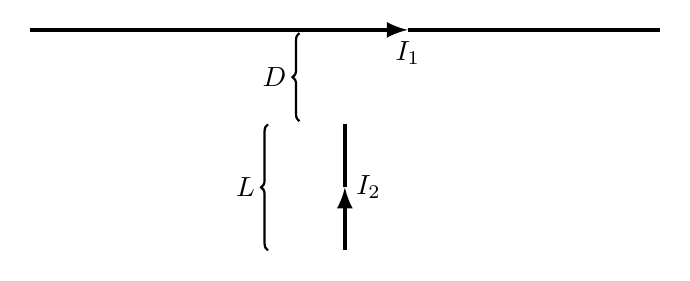
\begin{tikzpicture}[>=latex,scale=0.4]
    \draw[black, ultra thick, ->] (-10,5) -- (2,5) node[anchor=north] {$I_1$};
    \draw[black, ultra thick] (2,5) -- (10,5);
    \draw[black, ultra thick, ->] (0,-2) -- (0,0) node[anchor=west] {$I_2$};
    \draw[black, ultra thick] (0,0) -- (0,2);
	\draw[black, thick, decoration={brace,raise=5pt}, decorate] (-2,-2) -- (-2,2) node[black, midway, left=6pt] {$L$};
	\draw[black, thick, decoration={brace,raise=5pt}, decorate] (-1,2.1) -- (-1,4.9) node[black, midway, left=6pt] {$D$};
\end{tikzpicture}
\end{figure}

Calculate the force on wire 2 (the wire with current $I_2$) due to wire 1.

\end{frame}

\begin{frame}{Worked Example --- Forces on Current-Carrying Wires}

\textit{Solution.} We want the force \emph{on wire 2} from \emph{due to wire 1}. We start by noting that the magnitude of the magnetic field produced by an infinite wire is
\begin{equation*}
    B_{\text{inf. wire}} = \frac{\mu_o I}{2\pi\ r}
\end{equation*}

Furthermore, let's impose the following coordinate system:
\begin{figure}[H]
\centering
\begin{tikzpicture}[>=latex,scale=0.4]
    \draw[black, ultra thick, ->] (-10,0) -- (-2,0) node[anchor=north] {$I_1$};
    \draw[black, ultra thick] (-2,0) -- (10,0);
    \draw[black, ultra thick, ->] (0,-6) -- (0,-4) node[anchor=west] {$I_2$};
    \draw[black, ultra thick] (0,-4) -- (0,-2);
    \draw[red, ultra thick, ->] (0,0) -- (2,0) node[red, anchor=north west] {$x$};
    \draw[red, ultra thick, ->] (0,0) -- (0,2) node[red, anchor=south east] {$y$};
    \draw[red, thick] (0,0) circle (0.4);
    \node[red] at (-0.58,-0.58) {$z$};
    \node[red] at (4.8,2) {\parbox[c]{0.3\textwidth}{\begin{center} \tiny The origin of the coordinate system is directly above the wire stub. Note that the $z$-axis points out of the page. \end{center}}};
    \begin{scope}[scale=1,shift={(2,-4)}]
        \draw[BLUE] (0,0) circle (0.5);
        \draw[BLUE] (45:0.5) -- (225:0.5) node[BLUE, anchor=north west] {$\vec{B}_1$};
        \draw[BLUE] (135:0.5) -- (315:0.5);
    \end{scope}
    \node[BLUE] at (7,-4) {\parbox[c]{0.3\textwidth}{\begin{center} \tiny The magnetic field produced by the infinite wire points into the page in the vicinity of the wire stub. \end{center}}};
\end{tikzpicture}
\end{figure}

\end{frame}

\begin{frame}{Worked Example --- Forces on Current-Carrying Wires}

In this new coordinate system, the magnetic field produced by the infinite wire, in the vicinity of the wire stub, is
\begin{equation*}
    \vec{B}_1 = \frac{\mu_o\ I_1}{2\pi\ (-y)}\ \left( -\khat \right) = \frac{\mu_o\ I_1}{2\pi\ y}\ \khat
\end{equation*}

Nifty. Now observe that the wire stub points up on the page. As such, we can simply take $d\vec{\ell} = dy\ \jhat$. As such, the differential force exerted on the wire stub (the wire carrying current $I_2$) is
\begin{align*}
    d\vec{F} = I_2\ d\vec{\ell} \times \vec{B}_1 = \overbrace{I_2\ \left( dy\ \jhat \right)}^{I\ d\vec{\ell}} \times \overbrace{\left( \frac{\mu_o\ I_1}{2\pi\ y}\ \khat \right)}^{\vec{B}} = \frac{\mu_o\ I_1\ I_2}{2\pi\ y}\ dy\ \ihat
\end{align*}

(Note that $\jhat \times \khat = \ihat$ --- Think about the right-hand rule).

\end{frame}

\begin{frame}{Worked Example --- Forces on Current-Carrying Wires}

Now we just need to integrate to find the total force on wire 2. We're integrating with respect to $y$, so the lower and upper bounds of integration are the smallest and largest values of $y$, respectively.
\vspace{-2em}
\begin{align*}
    \vec{F} = \int d\vec{F} &= \int_{-(D+L)}^{-D} \frac{\mu_o\ I_1\ I_2}{2\pi\ y}\ dy\ \ihat \\
                            &= \frac{\mu_o\ I_1\ I_2}{2\pi} \int_{-(D+L)}^{-D} \frac{dy}{y}\ \ihat \\
                            &= \frac{\mu_o\ I_1\ I_2}{2\pi} \ln{\left( \frac{D}{D+L} \right)} \ihat
\end{align*}

By properties of logarithms, we can re-write this result as
\begin{equation*}
    \vec{F} = \frac{\mu_o\ I_1\ I_2}{2\pi} \ln{\left( \frac{D+L}{D} \right)} \left(-\ihat\right)
\end{equation*}

So the force on wire 2 is in the negative $x$-direction, as expected using the right-hand rule in conjunction with $d\vec{F} = I\ d\vec{\ell} \times \vec{B}$. $\blacktriangleleft$

\end{frame}

\begin{frame}{A Refresher on Torque}

Torque is given by
\begin{equation*}
    \vec{\tau} = \vec{r} \times \vec{F}
\end{equation*}

where $\vec{r}$ is the vector that points from the axis of rotation to the point of force application. If the applied force is non-uniform, we can instead consider the differential torque that comes from a differential force:
\begin{equation*}
    d\vec{\tau} = \vec{r} \times d\vec{F}
\end{equation*}

(Recall that just like a linear force $\vec{F}$ can be thought of a push, torque can be thought of as a twist about some axis).

\end{frame}

\begin{frame}{Worked Example --- Torque on a Slanted Wire}

$\blacktriangleright$ A wire carrying a current $I$ is free to rotate about the $y$-axis in the presence of a uniform magnetic field $\vec{B} = B_o\ \jhat$. What is the torque on the wire segment?

\begin{figure}[H]
\centering
\begin{tikzpicture}
    \draw[BLACK, ->] (-1,0) -- (5,0) node[BLACK, anchor=south west] {$x$};
    \draw[BLACK, ->] (0,-1) -- (0,5) node[BLACK, anchor=south west] {$y$};
    \draw[BLACK, ultra thick, ->] (0:0) -- (30:2.5) node[BLACK, anchor=south east] {$I$};
    \draw[BLACK, ultra thick, ->] (30:2.5) -- (30:5) node[BLACK, anchor=south west] {$I$};
    \draw[BLACK, <->] (0:1) arc (0:30:1) node[BLACK, pos=0.7, anchor=west] {$\theta$};
    \draw[BLUE, ultra thick, ->] (7,2) -- (7,4) node[BLUE, anchor=south] {$\vec{B_o}$};
\end{tikzpicture}
\end{figure}

\end{frame}

\begin{frame}{Worked Example --- Torque on a Slanted Wire}

\textit{Solution.} Here's our strategy: we'll start by first finding the differential amount of force with
\begin{equation*}
    d\vec{F} = I\ d\vec{\ell} \times \vec{B}
\end{equation*}

and then we'll get the $\vec{r}$-vector and get the differential amount of torque with
\begin{equation*}
    d\vec{\tau} = \vec{r} \times d\vec{F}.
\end{equation*}

Finally, we'll intergrate $d\vec{\tau}$ to find the total torque $\vec{\tau}$.

\end{frame}

\begin{frame}{Worked Example --- Torque on a Slanted Wire}

The differential amount of force is given by
\begin{equation*}
    d\vec{F} = I\ d\vec{\ell} \times \vec{B}
\end{equation*}

We have the magnetic field ($\vec{B} = B_o\ \jhat$). The infinitesimal length of the slanted wire segment is
\begin{equation*}
    d\vec{\ell} = dx\ \ihat + dy\ \jhat
\end{equation*}

We want everything in terms of $x$. So we leave $dx$ alone. To get $dy$ in terms of $dx$, recall that the segment in question is a line, with $\text{slope} = \frac{\text{rise}}{\text{run}} = \frac{L\sin{\theta}}{L\cos{\theta}} = \tan{\theta}$

\end{frame}

\begin{frame}{Worked Example --- Torque on a Slanted Wire}

Then it follows that $dy = \left( \text{slope} \right) dx = \tan{\theta}\ dx$. So the infinitesimal length of the slanted wire segment is
\begin{equation*}
    d\vec{\ell} = dx\ \ihat + \tan{\theta}\ dx\ \jhat
\end{equation*}

Taking the cross-product gives us
\begin{align*}
    d\vec{\ell} \times \vec{B} &= \begin{vmatrix} \ihat & \jhat & \khat \\ dx & \tan{\theta}\ dx & 0 \\ 0 & B_o & 0 \end{vmatrix} \\
    &= B_o dx\ \khat
\end{align*}

So the differential force vector is
\begin{equation*}
    d\vec{F} = I\ d\vec{\ell} \times \vec{B} = IB_o\ dx\ \khat
\end{equation*}

\end{frame}

\begin{frame}{Worked Example --- Torque on a Slanted Wire}

The differential torque vector is given by $d\vec{\tau} = \vec{r} \times d\vec{F}$. We already have $d\vec{F}$:
\begin{equation*}
    d\vec{F} = I\ d\vec{\ell} \times \vec{B} = IB_o\ dx\ \khat
\end{equation*}

The $\vec{r}$-vector points from the axis of rotation (the $y$-axis) to the point where force is being applied on the wire (so the $\vec{r}$-vector points straight to the right in the $\ihat$ direction). Its magnitude is given by the $x$-coordinate of the wire:
\begin{equation*}
    \vec{r} = x\ \ihat
\end{equation*}

So the final cross-product is
\begin{align*}
    d\vec{\tau} = \vec{r} \times d\vec{F} &= \begin{vmatrix} \ihat & \jhat & \khat \\ x & 0 & 0 \\ 0 & 0 & I B_o\ dx \end{vmatrix} \\
    &= -I B_o\ x\ dx\ \jhat
\end{align*}

\end{frame}

\begin{frame}{Worked Example --- Torque on a Slanted Wire}

We determined the differential torque vector to be
\begin{equation*}
    d\vec{\tau} = -I B_o\ x\ dx\ \jhat
\end{equation*}

We integrate to find the total torque. Since we're integrating with respect to $x$, the lower and upper bounds on the integral inherit the smallest and largest values of $x$, respectively.

\begin{align*}
    \vec{\tau} = \int d\vec{\tau} &= \int_0^{L\cos{\theta}} -I B_o\ x\ dx \\
                                  &= \boxed{\frac{-I B_o L^2 \cos^2{\theta}}{2} \jhat} \blacktriangleleft
\end{align*}

\end{frame}

\begin{frame}{Torque on a Current Loop}

If we have some current-carrying loop in a magnetic field (and only then), we can think of the torque on the loop in terms of the magnetic dipole instead. The magnetic dipole is given by
\begin{equation*}
    \vec{\mu} = NI\vec{A},
\end{equation*}

where $N$ is the number of turns, $I$ is the current, and $\vec{A}$ is the area vector. Recall that area vectors always point normal to the surface that they describe. Then the torque on the current-carrying loop is
\begin{equation*}
    \vec{\tau} = \underbrace{\left( NI\vec{A} \right)}_{\vec{\mu}} \times \vec{B}
\end{equation*}

\end{frame}

\begin{frame}{Motional EMF}

Sometimes, the \emph{motion} of charges through a magnetic field can \emph{induce} an emf. Let's take a look at the mechanics behind this.

\end{frame}

\begin{frame}{Motional EMF}

Suppose we have a conducting bar moving with velocity $\vec{v}$ in the presence of a magnetic field $\vec{B}$, as shown.

\begin{figure}[H]
\centering
\includegraphics[scale=0.2]{figures/motionalemf.png}
\end{figure}

\end{frame}

\begin{frame}{Motional EMF}

There are charges in the conducting bar. And those charges are \textcolor{GREENE}{moving} perpendicular to a \textcolor{BLUE}{magnetic field}. So those charges are subject to a \textcolor{RED}{force} given by
\begin{equation*}
    \Scale[1]{\RED \vec{F} \BLACK = \GREENE  q\vec{v} \BLACK \times \BLUE \vec{B}}
\end{equation*}

\vspace{-1.4em}

\begin{figure}[H]
\centering
\includegraphics[scale=0.16]{figures/memfmag.png}
\end{figure}

\vspace{-2em}

Consequently, positive charges are pushed to one end of the rod, leaving a residual negative charge at the other end. (The force $\vec{F}_B$ shown in the picture above is the force exerted on a positive charge --- the force on a negative charge is in the opposite direction.)

\end{frame}

\begin{frame}{Motional EMF}

This separation of charges sets up an electric field. Remember that electric fields always point from positive charges to negative charges.

\begin{figure}[H]
\centering
\includegraphics[scale=0.16]{figures/memfef.png}
\end{figure}

\end{frame}

\begin{frame}{Motional EMF}

So an equilibrium is established, with equal and opposite electric and magnetic forces.

\begin{figure}[H]
\centering
\includegraphics[scale=0.12]{figures/equilibrium.png}
\end{figure}

\vspace{-2.2em}

\begin{gather*}
    \overbrace{\left| q\vec{v} \times \vec{B} \right|}^{F_B} = \overbrace{\left| q\vec{E} \right|}^{F_E} \quad \implies \quad \cancel{q} vB = \cancel{q} E \quad \implies \quad E = vB
\end{gather*}

(As before, the forces $\vec{F}_E$ and $\vec{F}_B$ in the picture above are the electric and magnetic forces on a \emph{positive} charge, respectively. Both of these forces point in the opposite direction for negative charges.)

\end{frame}

\begin{frame}{Motional EMF}

As such, the charges are fixed in place and there's a voltage difference across the rod. This is known as a \emph{motional emf}.

\begin{figure}[H]
\centering
\includegraphics[scale=0.16]{figures/motionalvoltage.png}
\end{figure}

To determine this voltage difference, we integrate across the length of the bar:
\begin{equation*}
    \left| \Delta V \right| = \int \vec{E} \cdot d\vec{\ell} = \int E\ d\ell = \int (vB)\ d\ell = vBL
\end{equation*}

\end{frame}

\begin{frame}{Worked Example --- Motional EMF}

$\blacktriangleright$ A Boeing 787-8, with a wingspan of \SI{60.12}{\metre}, departed from the South Carolina final assembly and delivery facility. Once it reached its cruising speed of Mach 0.85 (\SI{903}{\kilo\metre/\hour}), it transversed a region where the Earth's magnetic field of \SI{6.0e-5}{\tesla} was directed \ang{10} downward from the horizontal. What is voltage difference across the aircraft's wingtips?

\vfill

\textit{Solution.} This is a motional emf problem, so let's consider what happens to the charges in the aircraft's wings.

\end{frame}

\begin{frame}{Worked Example --- Motional EMF}

The charges in the aircraft's wings are subject to a magnetic force:
\begin{equation*}
    \vec{F}_B = q\vec{v} \times \vec{B}
\end{equation*}

As the charges are pushed towards the ends of the wings, they set up an electric field. Thus, there's a competing electric force:
\begin{equation*}
    \vec{F}_E = q\vec{E}
\end{equation*}

An equilibrium will be established, which insinuates that the magnitudes of these two forces are equal:
\begin{gather*}
    \left| q\vec{v} \times \vec{B} \right| = \left| q\vec{E} \right| \\
    \cancel{q} v B \sin{\theta} = \cancel{q} E
\end{gather*}

where $\theta$ is the angle between the velocity $\vec{v}$ and the magnetic field $\vec{B}$ (this is the given angle of \ang{10}).

\end{frame}

\begin{frame}{Worked Example --- Motional EMF}

Thus, we have
\begin{equation*}
    E = vB\ \sin{\theta}
\end{equation*}

Integrating along the wingspan to get the voltage difference gives us
\begin{equation*}
    \left| \Delta V \right| = \int \vec{E} \cdot d\vec{\ell} = \int_{0}^{L} vB\ \sin{\theta}\ d\ell = vBL\ \sin{\theta}
\end{equation*}

\end{frame}

\begin{frame}{Worked Example --- Motional EMF}

Now we're just about ready to plug in numbers. Note that we have to convert the given velocity to SI-units:
\begin{equation*}
    \SI{903}{\kilo\metre/\hour} \cdot \frac{\SI{1000}{\metre}}{\SI{1}{\kilo\metre}} \cdot \frac{\SI{1}{\hour}}{\SI{3600}{\second}} = \SI{250.83}{\metre/\second} 
\end{equation*}

So the expected voltage difference is
\begin{gather*}
    \left| \Delta V \right| = \left( \SI{250.83}{\metre/\second} \right) \left( \SI{6.0e-5}{\tesla} \right) \left( \SI{60.12}{\metre} \right) \sin{\left( \ang{10} \right)} \\
    \implies \boxed{\big| \Delta V \big| = \SI{0.157}{\volt}} \blacktriangleleft
\end{gather*}

\end{frame}

\begin{frame}{Faraday's Law}

Faraday's law reads
\begin{equation*}
    \oint \left( \vec{E} + \vec{v} \times \vec{B} \right) \cdot d\vec{\ell} = -\frac{d}{dt} \left( \int \vec{B} \cdot d\vec{A} \right)
\end{equation*}

which is scary. Let's break it apart.

\end{frame}

\begin{frame}{Right-Hand Side of Faraday's Law}

The right-hand side of Faraday's law has the time-derivative of the magnetic flux through some surface:
\begin{equation*}
    \frac{d}{dt} \underbrace{\left( \int \vec{B} \cdot d\vec{A} \right)}_{\Phi_B} = \frac{d\Phi_B}{dt}
\end{equation*}

That surface could be \emph{any open surface}. A loop, for instance.

\end{frame}

\begin{frame}{Left-Hand Side of Faraday's Law}

The left-hand side of Faraday's law is a \emph{closed} line integral:
\begin{equation*}
    \oint \left( \vec{E} + \vec{v} \times \vec{B} \right) \cdot d\vec{\ell}
\end{equation*}

Let's break this integral apart at the addition:
\begin{equation*}
    \underbrace{\oint \vec{E} \cdot d\vec{\ell}}_{\parbox[c]{0.3\textwidth}{\vspace{-0.8em} \begin{center} \tiny This term asserts that integrals of \emph{curly} electric fields (those produced by changing magnetic fields) over a closed loop gives some voltage. Physically, this corresponds to, say, wiggling a magnet in a stationary loop. \end{center}}} \quad + \quad \underbrace{\oint \left( \vec{v} \times \vec{B} \right) \cdot d\vec{\ell}}_{\parbox[c]{0.3\textwidth}{\vspace{-0.8em}\begin{center} \tiny This term asserts that the motion of the loop itself also creates voltage. Physically, this corresponds to say, wiggling a loop near a stationary magnet. \end{center}}}
\end{equation*}

\end{frame}

\begin{frame}{Faraday's Law}

Altogether, it doesn't matter whether those voltages come from moving a magnet near a stationary loop or moving a loop near a stationary magnet. Either way, those are \emph{induced} voltages:
\begin{equation*}
    \oint \left( \vec{E} + \vec{v} \times \vec{B} \right) \cdot d\vec{\ell} = \text{emf}
\end{equation*}

We can therefore express Faraday's law in a much simpler form:
\begin{gather*}
    \oint \left( \vec{E} + \vec{v} \times \vec{B} \right) \cdot d\vec{\ell} = -\frac{d}{dt} \int \vec{B} \cdot d\vec{A} \\
    \Downarrow \\
    \text{emf} = -\frac{d\Phi_B}{dt}
\end{gather*}

Here, Faraday's law asserts that whenever the magnetic flux through an open surface changes \emph{for any reason}, there'll be an induced emf.

\end{frame}

\begin{frame}{Faraday's Law for Electromagnetic Induction}

For instance, the magnetic flux through the loop below is changing with time because of the \emph{motion of the loop}, even if the magnetic field itself is unchanged:

\begin{figure}[H]
\centering
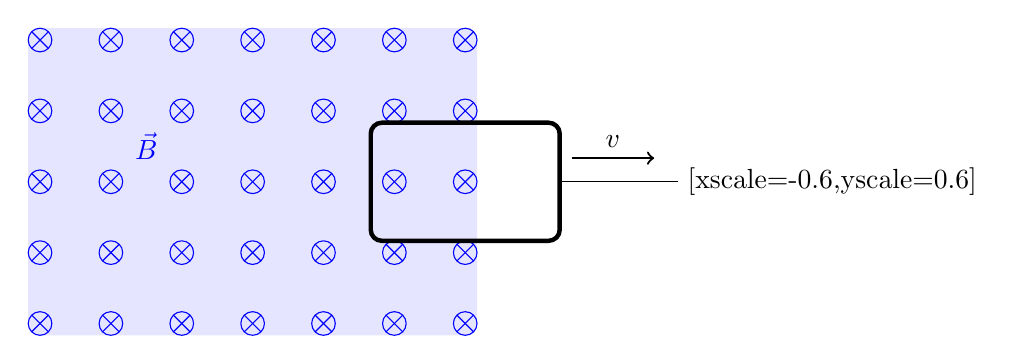
\begin{tikzpicture}[scale=0.15]
    \fill[blue!10, rounded corners] (-19, -13) rectangle (19, 13);
    \node[blue] at (-9,3) {$\vec{B}$};
    \foreach \x in {-18, -12, -6, 0, 6, 12, 18}
    \foreach \y in {-12, -6, 0, 6, 12}
    {
    \begin{scope}[shift={(\x,\y)}]
        \draw[blue] (0,0) circle (1);
        \draw[blue] (45:1) -- (225:1);
        \draw[blue] (135:1) -- (315:1);
    \end{scope}
    }
    \draw[black, ultra thick, rounded corners] (10,-5) rectangle (26,5);
    \draw[black] (26,0) -- (36,0) node[black, right]{\okay[xscale=-0.6,yscale=0.6]};
    \draw[black, thick, ->] (27,2) -- (34,2) node[black, midway, above] {$v$};
\end{tikzpicture}
\end{figure}

\end{frame}

\begin{frame}{Faraday's Law for Electromagnetic Induction}

Another possibility is when the magnetic field itself changes with time:

\begin{columns}

\begin{column}{0.5\textwidth}
\begin{figure}[H]
\centering
\includegraphics[width=\textwidth]{figures/increasing_bfield_init.png}
\end{figure}
\end{column}
~
\begin{column}{0.5\textwidth}
\hspace{4em}
\begin{figure}[H]
\centering
\includegraphics[width=\textwidth]{figures/increasing_bfield_fin.png}
\end{figure}
\end{column}

\end{columns}

\vfill

The changing magnetic flux through the loop induces an emf.

\end{frame}

\begin{frame}{Lenz's Law}

When a thing (current, emf, or a $\vec{B}$-field) is being induced by Faraday's law, that thing will act in such a way as to oppose the change that caused it.
    
\end{frame}

\begin{frame}{Worked Example --- A Rectangular Coil}

A rectangular coil sits in the $xy$-plane as shown below. It has width $a$ and height $b$ and 32 turns. There is a spatially-varying magnetic field pointing out of the page (in the positive $z$-direction) whose magnitude is $B = 4x\ e^{-3t}$.

\begin{figure}[H]
\centering
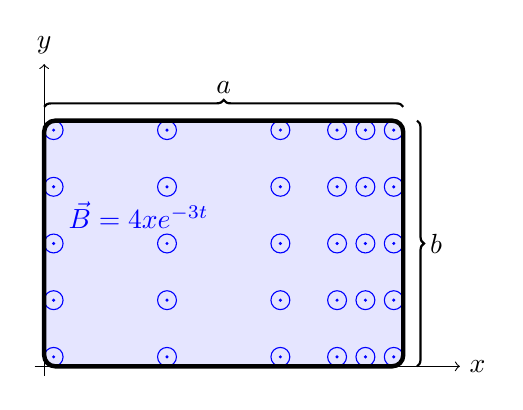
\begin{tikzpicture}[scale=0.12]
    \draw[black, ->] (-20,-13) -- (25,-13) node[black, anchor=west] {$x$};
    \draw[black, ->] (-19,-14) -- (-19,19) node[black, anchor=south] {$y$};
    \fill[blue!10, rounded corners] (-19, -13) rectangle (19, 13);
    \node[blue] at (-9,3) {$\vec{B} = 4x e^{-3t} \khat$};
    \foreach \x in {-18, -6, 6, 12, 15, 18}
    \foreach \y in {-12, -6, 0, 6, 12}
    {
    \begin{scope}[shift={(\x,\y)}]
        \draw[blue] (0,0) circle (1);
        % \draw[blue] (45:1) -- (225:1);
        % \draw[blue] (135:1) -- (315:1);
		\filldraw[blue] (0,0) circle (0.1);
    \end{scope}
    }
    \draw[black, ultra thick, rounded corners] (-19,-13) rectangle (19,13);
	\draw[black, thick, decoration={brace, raise=5pt, mirror}, decorate] (19,-13) -- (19,13) node[black, midway, right=6pt] {$b$};
	\draw[black, thick, decoration={brace, raise=5pt}, decorate] (-19,13) -- (19,13) node[black, midway, above=6pt] {$a$};
\end{tikzpicture}
\end{figure}

Find the magnitude of the induced emf in the coil and find the direction of the induced current.

\end{frame}

\begin{frame}{Worked Example --- A Rectangular Coil}

    \textit{Solution.} We will apply Faraday's law, which asserts that the induced emf (through one turn of the loop) is
\begin{equation*}
	\mathcal{E} = -\frac{d\Phi_B}{dt}
\end{equation*}

So the magnitude of the induced emf in the entire coil is
\begin{equation*}
	\left| \mathcal{E} \right| = N \cdot \frac{d\Phi_B}{dt}
\end{equation*}

\begin{center}
    So let's start by finding the flux through one turn of the coil.
\end{center}

\end{frame}

\begin{frame}{Worked Example --- A Rectangular Coil}

The most general expression for the magnetic flux is
\begin{equation*}
	\Phi_B = \int \vec{B} \cdot d\vec{A}
\end{equation*}

We know that the magnetic field is
\begin{equation*}
	\vec{B} = 4x e^{-3t}\ \khat
\end{equation*}

What about the differential area vector $dA$? Since the rectangular coil seems to lie in the $xy$-plane, the differential area vector is
\begin{equation*}
	d\vec{A} = dx\ dy\ \khat
\end{equation*}

Why the $\khat$? Recall that area vectors are always perpendicular to the area that they describe, and the $\khat$ vector is perpendicular to the $xy$-plane.

\end{frame}

\begin{frame}{Worked Example --- A Rectangular Coil}

Now let's take the dot product. We have
\begin{gather*}
	\vec{B} \cdot d\vec{A} = \left( 4x e^{-3t}\ \khat \right) \cdot \left( dx\ dy\ \khat \right) = 4x\ e^{-3t}\ dx\ dy
\end{gather*}

(Note that $\khat \cdot \khat = 1$.) Now we're ready to integrate! The flux through one turn of the rectangular coil is
\begin{align*}
	\Phi_B = \int \vec{B} \cdot d\vec{A} &= \int_0^b \int_0^a 4x\ e^{-3t}\ dx\ dy \\
	&= 4 e^{-3t} \underbrace{\left( \int_0^b dy \right)}_{b} \underbrace{\left( \int_0^a x dx \right)}_{a^2/2} \\
	&= 2ba^2 e^{-3t}
\end{align*}

\end{frame}

\begin{frame}{Worked Example --- A Rectangular Coil}

Finally, we can apply Faraday's law (that is, take a time derivative) to find the induced emf. The magnitude of the induced emf in the entire coil is therefore
\begin{equation*}
    \left| \mathcal{E} \right| = \left| -N \frac{d\Phi_B}{dt} \right| = \left| -N \frac{d}{dt} \left( 2ba^2 e^{-3t} \right) \right| = 6 Nba^2 e^{-3t}
\end{equation*}

So the magnitude of the induced emf, as a function of time, is
\begin{equation*}
	\boxed{\mathcal{E}(t) = 6Nba^2 e^{-3t}}
\end{equation*}

\end{frame}

\begin{frame}{Worked Example --- A Rectangular Coil}

Now we need to determine the direction of the induced current. This is where Lenz's law becomes incredibly useful. In fact, Lenz's law asserts that the induced current will be in a direction opposite to the change that caused it.

\vfill

Note that the magnetic field initially points \emph{out of the page}. And since the magnetic field assumes the form $\vec{B} = 4x e^{-3t}\ \khat$, as time progresses the magnetic field points \emph{less out of the page} --- so the change that caused the induction was a magnetic field that points \emph{less out out the page}.

\vfill

As such, the induced current must oppose this change. In fact, the induced current must be \emph{counterclockwise}. On its own, a counterclockwise current will produce a magnetic field that points \emph{more out the page}.

\vfill

Thus, the induced current is \emph{counterclockwise}. $\blacktriangleleft$

\end{frame}

\begin{frame}{Mutual Inductance}

For a pair of coils, the mutual inductance is the quantity that relates how the the current in one coil affects the flux in the other:
\begin{equation*}
    M = \overbrace{N_2\ \Phi_{B, \text{ one turn of 2}}}^{\text{total flux in 2}} / I_1
\end{equation*}

Inductance is measured in \textbf{Henries} (H):
\begin{equation*}
\SI{1}{\henry} = \SI{1}{\frac{\tesla\cdot\metre^2}{\ampere}} = \SI{1}{\joule/\ampere^2}
\end{equation*}

And Faraday's law tells us that we can take the time-derivative of magnetic flux to find the induced emf. As such, the induced emf is
\begin{equation*}
    \mathcal{E}_1 = -M \frac{dI_2}{dt} \qquad \Longleftrightarrow \qquad \mathcal{E}_2 = -M \frac{dI_1}{dt}
\end{equation*}

\end{frame}

\begin{frame}{Worked Example --- Solenoid Through a Coil}

$\blacktriangleright$ A long solenoid of length $L = \SI{18.5}{\centi\metre}$ has $N_a = 25$ windings and a cross-sectional radius $a = \SI{1.90}{\centi\metre}$. The solenoid goes through the center of a circular coil of wire with $N_b = 31$ windings and radius $b = \SI{5.50}{\centi\metre}$. The current in the circular coil changes according to $I(t) = 7.0 t^2 + 1.0 t$. What is the magnitude of the induced emf in the solenoid at $t = \SI{3.00}{\second}$?

\begin{figure}[H]
\centering
\includegraphics[height=0.5\textheight]{figures/solenoid_and_loop.png}
\end{figure}

\end{frame}

\begin{frame}{Worked Example --- Solenoid Through a Coil}

\textit{Solution.} We'll start by finding the mutual inductance for this pair of coils. Then we'll use Faraday's law to determine the induced emf in the solenoid at some time $t$.

\end{frame}

\begin{frame}{Worked Example --- Solenoid Through a Coil}

The mutual inductance of a pair of coils is given as
\begin{equation*}
    M = N_2\ \Phi_{B, \text{ one turn of 2}} / I_1
\end{equation*}

This means either treating the coil as producing the magnetic field and finding the flux through the solenoid:
\begin{equation*}
    M = \frac{N_{\text{solenoid}} \Phi_{B, \text{ one turn of solenoid}}}{I_{\text{coil}}}
\end{equation*}

Or treating the solenoid as producing the magnetic field and finding the flux through the coil:
\begin{equation*}
    M = \frac{N_{\text{coil}} \Phi_{B, \text{ one turn of coil}}}{I_{\text{solenoid}}}
\end{equation*}

\end{frame}

\begin{frame}{Worked Example --- Solenoid Through a Coil}

By far the easier approach is to find the flux through the coil. Recall that a solenoid has a nearly-uniform magnetic field within itself:
\begin{equation*}
    B_{\text{solenoid}} = \mu_o n I
\end{equation*}

and nearly zero magnetic field outside itself:

\begin{figure}[H]
\centering
\includegraphics[height=0.5\textheight]{figures/solenoid_bfield.png}
\end{figure}

\end{frame}

\begin{frame}{Worked Example --- Solenoid Through a Coil}

The flux through one turn of the coil is
\begin{equation*}
    \Phi_{B} = \int \vec{B} \cdot d\vec{A} = B \cdot A = \left( \mu_o n I_{\text{solenoid}} \right) \cdot \left( \pi a^2 \right)
\end{equation*}

Be super careful here! Even though we're considering the flux through the coil --- which has an area of $\pi b^2$ --- the magnetic field is zero outside the solenoid! That is, the only part of the coil's area through which there is a non-zero flux is the part that containts the solenoid.

\vfill

The mutual inductance is then
\begin{equation*}
    M = \frac{N_b \overbrace{\left( \mu_o \frac{N_a}{L} I_{\text{solenoid}} \right) \left( \pi a^2 \right)}^{\Phi_{B, \text{ one turn of coil}}}}{I_{\text{solenoid}}} = \frac{\mu_o N_a N_b \pi a^2}{L} = \SI{5.97e-6}{\henry}
\end{equation*}

\end{frame}

\begin{frame}{Worked Example --- Solenoid Through a Coil}

Now that we have the mutual inductance, we can find the induced emf in the solenoid at some time $t$ via
\begin{equation*}
    \mathcal{E}_{\text{solenoid}} = -M \frac{dI_{\text{coil}}}{dt}
\end{equation*}

The current in the coil is given as $I(t) = 7.0 t^2 + 1.0 t$, so $\frac{dI}{dt} = 14.0 t + 1.0$. And so the magnitude of the induced emf in the coil at some time $t$ is
\begin{equation*}
    \mathcal{E}_{\text{solenoid}} = \overbrace{\left( \frac{\mu_o N_a N_b \pi a^2}{L} \right)}^{M} \underbrace{\left( 14.0 t + 1.0 \right)}_{\frac{dI}{dt}}
\end{equation*}

In particular, at $t= \SI{3.00}{\second}$, the induced emf in the solenoid is
\begin{equation*}
    \boxed{\mathcal{E}_{\text{solenoid}} \bigg|_{t=3.00} = \SI{2.57e-4}{\volt}} \blacktriangleleft
\end{equation*}

\end{frame}

\begin{frame}{Self Inductance}

Solenoids or coils of wire can even create a magnetic flux through itself! Consider, for instance, a current-carrying solenoid with radius $R$, length $\ell$, and $N$ number of turns:

\begin{figure}[H]
\centering
\includegraphics[height=0.45\textheight]{figures/solenoid.png}
\end{figure}

The magnetic field inside a solenoid is
\begin{equation*}
    B_{\text{solenoid}} = \mu_o n I = \mu_o \left( \frac{N}{\ell} \right) I
\end{equation*}

\end{frame}

\begin{frame}{Self Inductance}

The total flux through the solenoid is therefore
\begin{gather*}
    \Phi_B = \int \vec{B} \cdot d\vec{A} = B \cdot A = \left[ \mu_o \left( \frac{N}{\ell} \right) I \right] \cdot \left[ N \pi R^2 \right] \\[1em]
    \implies \Phi_B = \underbrace{\left( \frac{\mu_o N^2 \pi R^2}{\ell} \right)}_{L} I
\end{gather*}

\vfill

That quantity $L$ is known as the \emph{self-inductance} of the solenoid, and it plays a similar role to mutual inductance (without the other coil, of course).

\end{frame}

\begin{frame}{Self Inductance}

In fact, we can apply Faraday's law (that is, take the time-derivative of the flux) to find the induced emf:
\begin{equation*}
    \mathcal{E} = -\frac{d\Phi_B}{dt} = -\frac{d}{dt} \left( LI \right) = -L \frac{dI}{dt}
\end{equation*}

So inductors \emph{oppose changes in current} through them.

\vfill

\begin{center}
Un-energized inductors (when current gets turned on suddenly) act like open switches
\end{center}

\begin{center}
Energized inductors (when current has been flowing for a long time) act like ideal wires.
\end{center}

\end{frame}

\begin{frame}{Worked Example --- Inductors in a Circuit}

$\blacktriangleright$ Consider the following circuit:

\begin{figure}[H]
\centering
\begin{circuitikz}
    \draw (0,0) to[resistor,l^=$R_3$] (0,2);
    \draw (0,2) to[switch] (0,4);
    \draw (0,0) to (3,0);
    \draw (0,4) to[battery,l^=$V$] (3,4);
    \draw (3,0) to[capacitor,l^=$C$] (3,1.3);
	\draw (3,1.3) to[inductor,l^=$L_2$] (3,2.6);
	\draw (3,2.6) to[resistor,l^=$R_2$] (3,4);
    \draw (3,0) to (6,0);
    \draw (3,4) to (6,4);
    \draw (6,0) to[inductor,l^=$L_1$] (6,2.4);
    \draw (6,2) to[resistor,l^=$R_1$] (6,4);
\end{circuitikz}
\end{figure}

Assume that $R_1 > R_2 > R_3$. Rank the currents in through the three resistors after the switch has been closed for a very long time.

\end{frame}

\begin{frame}{Worked Example --- Inductors in a Circuit}

\textit{Solution.} This problem isn't going to require any math --- instead, we can just recall that inductors oppose changes in current through them to solve this problem.

\vfill

So in this case, the current has been on for a long time, meaning that an inductor would act like an ideal wire. However, we also have a capacitor. And capacitors do the opposite --- a charged capacitor acts like a open switch, meaning there is no current in that entire middle segment.

\vfill

So resistors 1 and 3 have the same current, and resistor 2 has zero current after the switch has been closed for a long time. $\blacktriangleleft$

\end{frame}

\begin{frame}{LR Circuits}

Inductor-Resistor circuits, also known as LR circuits, are similar to the RC circuits we studied earlier:
\begin{equation*}
    \underbrace{I(t) = I_{\text{final}} \left( 1 - e^{-t/(L/R)} \right)}_{\parbox[c]{0.4\textwidth}{\begin{center} There's some emf source in the circuit and the current reaches some final value as time $t$ approaches infinity \end{center}}} \qquad\qquad \underbrace{I(t) = I_{\text{initial}} e^{-t/(L/R)}}_{\parbox[c]{0.4\textwidth}{\begin{center} There is no emf source in the circuit and the current decays to zero as time $t$ approaches infinity \end{center}}}
\end{equation*}

\end{frame}

\end{document}
